% !TEX root=../index.tex

\chapter{Validazione e Testing dei Classificatori}
\label{chap:tuning}
    Al termine della fase di allenamento si ottengono dei classificatori della forma: 
    \begin{equation}\tag{\ref{eq:strong_classifier}}
        F(x) = 
        \begin{cases}
            1 & \text{ se } \sum_{t = 1}^{T} \alpha_t h_t(x) > \theta \sum_{t = 1}^{T} \alpha_t \\
            0 & \text{ altrimenti }
        \end{cases}
    \end{equation}
    La valore di soglia $\theta$, a questo punto, è ancora ignoto e dovrà essere fissato in modo tale da massimizzare le prestazioni del sistema. È necessario, inoltre, impostare il corretto numero di \emph{weak learner} per ogni \emph{strong learner}, al fine di evitare problemi di \emph{overfitting}.
    
    Queste operazioni sono volte alla \emph{validazione} dei vari classificatori e devono essere affiancate da opportune operazioni di \emph{testing} per la valutazione complessiva del sistema.

    \section{Criteri di Valutazione}
    \label{sec:evaluation_criteria}
        Applicando i vari classificator ad un set di elementi si può visualizzare la distribuzione delle istanze degli oggetti rispetto alla classificazione predetta dai classificatori e rispetto a quella reale.

        Si utilizza la \emph{matrice di confusione} per descrivere in modo compatto tale distribuzione.

        \begin{definition}[Matrice di Confusione]
            In un generico problema di classificazione ad $n$ classi per il quale è definito un insieme di \emph{label} $L = \{l_1,..., l_n\}$ ed è stato allenato un classificatore $F(x)$, sia $T = \{(x_1,y_1),..., (x_m, y_m)\}$ un insieme di elementi per cui è nota la reale classificazione.

            Si chiama \emph{matrice di confusione} del classificatore $F$ e relativa all'insieme di elementi $T$, la matrice $C \in \mathbb{N}^{n \times n}$, per cui ogni elemento $c_{ij}$ è pari al numero di oggetti dell'insieme $T$ la cui reale etichettatura corrisponde a $l_i$ e per i quali il classificatore $F(x)$ prevede l'etichettatura $l_j$.
            \begin{equation}
            \label{subeq:confusion_matrix_element}
                 c_{ij} = \#(\{x|(x,l_i) \in T \wedge F(x) = l_j\})
            \end{equation} 
        \end{definition}

        Gli elementi sulla diagonale principale di tale matrice denotano il numero di elementi per cui la predizione fornita dal classificatore è corretta. Infatti, nel caso in cui $i = j$, la relazione \ref{subeq:confusion_matrix_element} diventa:
        \begin{equation}
            c_{ii} = \#(\{x|(x,l_i) \in T \wedge F(x) = l_i\}) \Longrightarrow c_{ii} = \#(\{x|(x,F(x)) \in T\})
        \end{equation}

        Nel caso di classificazione dicotomica, la struttura della matrice di confusione è molto semplice:
        \begin{equation}\label{eq:confusion_matrix}
            C = \left(
            \begin{array}{cc}
            \text{True Positives} & \text{False Negatives}\\
            \text{False Positives} & \text{True Negatives}
            \end{array} \right)
        \end{equation}

        \subsection{Modalità di Test} % (fold)
        \label{sub:dataset_di_validazione}
            % Descrizione delle possibili alternative
            La scelta del set di elementi con i quali testare i classificatori, in fase di valutazione, è particolarmente importante. Esistono alcune alternative:
            \begin{description}
                \item [Training Dataset] Si utilizza lo stesso dataset impiegato per allenare il costruttore. È la soluzione più semplice, ma presenta notevoli svantaggi, in quanto diventa impossibile rilevare ed evitare problemi di \emph{overfitting}.

                \item [Validation Dataset] Si crea un dataset da utilizzare esclusivamente per il testing o per la validazione che non contenga elementi dell'insieme di allenamento.

                \item [Cross Validation] Questa tecnica prevede l'utilizzo di un unico dataset, utilizzato sia per l'allenamento che per la valutazione:
                \begin{enumerate}
                    \item Si suddivide l'insieme in $k$ sottoinsiemi, detti \emph{k-fold}\footnote{Si è notato che, sperimentalmente, sono sufficienti una decina di \emph{fold}.}
                    \item Il classificatore viene allenato utilizzando $k-1$ sottoinsiemi e viene testato utilizzando il sottoinsieme rimanente. Questa operazione viene eseguita $k$ volte.
                    \item La media delle singole prestazioni ottenute nei $k$ esperimenti costituisce le prestazioni complessive del sistema.
                \end{enumerate}

                \item [Split] Si suddivide l'insieme di dati disponibili in due set distinti, uno da utilizzare per l'allenamento, l'altro - solitamente più piccolo del primo - per la validazione e per il testing.
            \end{description}

            % Traiettorie Causali
            Per la validazione e per il testing è stato creato un dataset apposito, estratto da registrazioni completamente diverse da quelle utilizzate per i dataset di allenamento.
            Le porzioni di immagine di profondità che ritraggono la figura della persona, in questo dataset, provengono dalle registrazioni in cui i vari soggetti percorrono delle traiettorie a loro piacimento all'interno dell'area d'interesse.

            % Dimensioni e Negativi
            Il dataset di validazione è costituito da 1500 elementi positivi (immagini che ritraggono persone) e da 1600 elementi negativi.
        % subsection dataset_di_validazione (end)

        \subsection{Misure per Valutare le Prestazioni} % (fold)
        \label{sub:misure_per_valutare_le_prestazioni}
            Scegliere i criteri di valutazione della bontà delle previsioni fornite dai classificatori è un punto cruciale e non banale: l'utilizzo di una misura piuttosto che un'altra dipende dall'obiettivo che si vuole raggiungere.

            Per i problemi di classificazione binaria sono disponibili le seguenti misure per valutarne le prestazioni.
            \begin{description}
                \item [Precision] Porzione di predizioni positive corrette.
                \begin{equation}
                    \label{eq:precision}
                    PR = \frac{TP}{TP + FP}
                \end{equation}

                \item [Sensitiviy o Recall] Porzione delle istanze realmente positive classificate correttamente. Per $P$ si intende il numero totale di istanze realmente positive.
                \begin{equation}
                    \label{eq:tpr}
                    TPR = \frac{TP}{P} = \frac{TP}{TP + FN}
                \end{equation}

                \item [Specificity] Porzione di istanze realmente negative classificate correttamente. Per $N$ si intende il numero totale di istanze negative.
                \begin{equation}
                    \label{eq:tnr} 
                    TNR = \frac{TN}{N} = \frac{TN}{TN + FP}
                \end{equation}

                \item [False Positive Rate] Porzione di istanze realmente negative classificate erroneamente come positive.
                \begin{equation}
                    \label{eq:fpr}
                    FPR = \frac{FP}{N} = \frac{FP}{TN + FP} = 1 - TNR
                \end{equation}

                \item [Accuracy] Porzione di istanze, sia positive che negative, classificate correttamente.
                \begin{equation}
                    \label{eq:accuracy}
                    ACC = \frac{TP+TN}{P + N} = \frac{TP + TN}{TP + TN + FP + FN}
                \end{equation}

                \item [F1 measure] Media armonica tra \emph{precision} e \emph{recall}.
                \begin{equation}
                    \label{eq:f1_measure}
                    F1 = \frac{2PR\cdot TPR}{PR + TPR} = \frac{2TP}{2TP + FP + FN}
                \end{equation}
            \end{description}

        \emph{F1 measure} e \emph{accuracy} sono le misure più indicate per la valutazione complessiva dei classificatori, mentre le altre forniscono informazioni parziali.

        Solitamente si utializzano \emph{precision}, \emph{recall} e \emph{F1 measure}, nei problemi in cui, tra le due classi, una è molto meno interessante dell'altra, oppure nei casi in cui si vuole studiare l'andamento del classificatore nelle predizioni di una classe di oggetti in particolare.

        D'altra parte, l'\emph{accuracy} viene utilizzata quando tutte le classi ricoprono una posizione di egual interesse. 
        In particolare, nei problemi binari, tale misura è una adeguata fonte di valutazione quando le due classi sono bilanciate.

        In questa applicazione, poichè le classi e la distribuzione degli elementi di allenamento rispettano i criteri di quest'ultima misura, verrà utilizzata l'\emph{accuracy} come misura di valutazione delle prestazioni.
        
        % subsection misure_per_valutare_le_prestazioni (end)

    \section{Massimizzazione all'\emph{Accuracy}}
    \label{sec:accuracy_maximization}
        \subsection{Parametri liberi del classificatore}
        I classificatori allenati con Adaboost non sono ancora pronti per poter essere utilizzati, vi sono ancora dei parametri liberi da vincolare.
        Dal momento che l'obiettivo è ottenere un sistema di rilevamento che sia più accurato possibile, questi parametri devono essere impostati in modo tale che l'\emph{accuracy} sia massima.
            \subsubsection{Numero di weak learner}
                Il numero di weak learner\footnote{Abbreviando: NWL} per ogni classificatore forte è un parametro libero all'interno della procedura di allenamento.
                Vista la procedura di Adaboost nel capitolo precedente, potrebbe sembrare che, aggiungendo altri weak learner si possa migliorare progressivamente la precisione del sistema.
                Ciò generalmente non è vero: troppi classificatori deboli potrebbero generare problemi di \emph{overfitting}.
                È necessario quindi ricavare il numero ottimale di classificatori deboli a comporre ciascun classificatore forte.

            \subsubsection{Soglia del classificatore}
                Il valore di soglia relativo a ciascun classificatore forte allenato non è mai stato precisato.
                È necessario quindi impostare tale valore al fine di migliorare complessivamente l'affidabilità del sistema.

        \subsection{Algoritmo di ricerca della soglia e del NWL ottimi}
            I parametri da definire sono quindi il numero di classificatori deboli ed il valore di soglia per ciascuno dei classificatori forti allenati.
            Entrambi vengono scelti, per ogni classificatore forte, al fine di massimizzarne l'accuratezza in relazione al dataset di validazione.
            Ciò implica la massimizzazione del numero di oggetti che vengono classificati correttamente e la conseguente riduzione dei falsi positivi e negativi.

            L'algoritmo per determinare tali valori è fondamentalmente semplice: ogni strong learner viene utilizzato per classificare gli elementi del \emph{dataset di validazione}.
            L'attività di classificazione, in virtù dei parametri liberi appena identificati, sarà dipendente dalla coppia di valori $(\theta, N_{wl})$ \footnote{Per $\theta$ si intende il valore di soglia del classificatore e $N_{wl}$ il numero di weak learner che lo compongono}.
            Per ogni possibile coppia di parametri, viene misurata l'accuratezza del classificatore nel classificare correttamente l'intero dataset, quindi viene scelta la coppia per cui l'accuratezza è massima.

            Una procedura di questo tipo, se implementata senza adoperare dei piccoli accorgimenti, potrebbe richiedere molto tempo per essere portata a termine.
            Di seguito viene presentato un metodo che permette di classificare molto velocemente il dataset di validazione utilizzando diversi valori per la coppia $(\theta, N_{wl})$.

            \begin{enumerate}
                \item Si definisce il classificatore forte $F(x)$ (equazione \ref{eq:strong_classifier}) costituito dai primi $T$  weak learner\footnote{In questa applicazione vengono estratti i primi 200 classificatori deboli. Questi ultimi sono il limite superiore al numero di weak learner totali che potranno essere utilizzati.}, selezionati da Adaboost.

                \item Si definisce l'insieme $V = {(x_1, y_1),..., (x_m, y_m)}$ di validazione.

                \item Si costruisce la matrice di valutazione dei weak learner $W$. L'elemento alla posizione $(i,j)$ di tale matrice sarà la valutazione del \emph{j-esimo weak lerner} sul \emph{i-esimo elemento del dataset}.
                \begin{equation}
                    \label{subeq:wl_valuation_matrix}
                    W = \left[
                    \begin{array}{cccccc}
                        h_1(x_1) & h_2(x_1) & \cdots & h_j(x_1) & \cdots & h_T(x_1)\\
                        h_1(x_2) & h_2(x_2) & \cdots & h_j(x_2) & \cdots & h_T(x_2)\\
                        \vdots & \vdots & & \vdots & & \vdots \\
                        h_1(x_i) & h_2(x_i) & \cdots & h_j(x_i) & \cdots & h_T(x_i)\\
                        \vdots & \vdots & & \vdots & & \vdots \\
                        h_1(x_m) & h_2(x_m) & \cdots & h_j(x_m) & \cdots & h_T(x_m)\\
                    \end{array}
                    \right]
                \end{equation}
                Poichè $h_j(x_i): V \rightarrow \{0,1\}$, allora tale matrice sarà composta solamente da $0$ ed $1$ (con un piccolo abuso di notazione: $W \in \{0,1\}^{m \times T}$).

                \item Si costruisce una matrice triangolare superiore con i moltiplicatore dei weak learner, disposti come di seguito:
                \begin{equation}
                    \label{subeq:wl_multipliers_matrix}
                    A = \left[
                    \begin{array}{cccccc}
                        \alpha_1 & \alpha_1 & \cdots & \alpha_1 & \cdots & \alpha_1 \\
                        0 & \alpha_2 & \cdots & \alpha_2 & \cdots & \alpha_2 \\
                        \vdots & \vdots & \ddots & \vdots & & \vdots \\
                        0 & 0 & \cdots & \alpha_i & \cdots & \alpha_i \\
                        \vdots & \vdots & & \vdots  & \ddots & \vdots \\
                        0 & 0 & \cdots & 0 & \cdots & \alpha_T
                    \end{array}
                    \right] \in \mathbb{R}^{T \times T}
                \end{equation}

                \item Si calcola il prodotto della matrice $W$ e della matrice $A$. L'elemento alla posizione $(i,j)$ della matrice risultante, sarà il \emph{valore della combinazione lineare dei primi j weak learner, valutati sul i-esimo elemento del dataset di validazione}.
                \begin{equation}
                    \label{subeq:wca}
                    \forall a_{ij} \in (W \cdot A), 
                    a_{ij} = \sum_{t = 1}^{j} a_t h_t(x_i)
                \end{equation}

                \item Si definiscono i possibili valori di soglia assumibili dal classificatore forte. Qui sono stati utilizzati tutti i valori da $0$ ad $1$, con un passo pari a $0.01$, estremi inclusi\footnote{Quindi i possibili valori di soglia sono 101: $\{0, 0.01, 0.02, ..., 0.98, 0.99, 1\}$}.
                \begin{equation}
                    \label{subeq:thresholds_vector}
                    \Theta = \left[
                    \begin{array}{c}
                        \theta_1 \\
                        \theta_2 \\
                        \vdots \\
                        \theta_l \\
                    \end{array}
                    \right] \in \mathbb{R}^l
                \end{equation}

                \item Si definisce un array con la somma cumulativa dei fattori moltiplicativi dei weak learner:
                \begin{equation}
                    \label{subeq:multipliers_cum_sum}
                    \widetilde{A} = \left[
                    \begin{array}{c}
                        \alpha_1 \\
                        \alpha_1 + \alpha_2 \\
                        \vdots \\
                        \sum_{t = 1}^{T} \alpha_t \\
                    \end{array}
                    \right] \in \mathbb{R}^T
                \end{equation}

                \item \emph{For} $i = [1...l]$ (ovvero, per ogni possibile valore di soglia):
                \begin{enumerate}

                    \item \emph{For} $t = [1...T]:$
                    \begin{enumerate}
                        
                        \item Si inizializzano $TP = TN = FP = FN = 0$.

                        \item \emph{For} $k = [1...m]$ (cioè, per ogni elemento del dataset di validazione):
                            \begin{enumerate}
                                
                                \item Si classifica velocemente l'elemento utilizzando le strutture dati preparate in precedenza:
                                \begin{equation}
                                    \label{subeq:element_fast_classification}
                                    F(x_k) = 
                                    \begin{cases}
                                        1 & \text{ se } a_{kt} > \theta_i \widetilde{a_t} \\
                                        0 & \text{ altrimenti }
                                    \end{cases}
                                \end{equation}

                                \item Si confronta tale classificazione con la classificazione reale e si aggiornano i contatori:
                                    \begin{itemize}
                                        \item $F(x_k) = y_k = 1 
                                        \Longrightarrow TP \leftarrow TP + 1$
                                        \item $F(x_k) = y_k = 0
                                        \Longrightarrow TN \leftarrow TN + 1$
                                        \item $F(x_k) = 1 \wedge y_k = 0 
                                        \Longrightarrow FP \leftarrow FP + 1$
                                        \item $F(x_k) = 0 \wedge y_k = 1 
                                        \Longrightarrow FN \leftarrow FN + 1$
                                    \end{itemize}

                                \item Si salvano i valori $TP, TN, FP, FN$ relativi alla coppia $(\theta_i, N_{wl})$ (con $N_{wl} = t$), organizzandoli in una struttura dati a piacere, purchè in un secondo momento si sia in grado di risalire esattamente al valore di soglia e al numero di weak learner utilizzati.

                                In questo caso, ad esempio, sono state utilizzate 4 matrici distinte, formate da tante colonne quanti sono i weak learner totali e da tante righe quanti sono i possibili valori di soglia.
                            \end{enumerate}
                    \end{enumerate}
                \end{enumerate}

                \item Per ogni coppia $(\theta, N_{wl})$ calcolare l'\emph{accuracy} (formula \ref{eq:accuracy}).
                Si seleziona la coppia di valori per i quali l'accuratezza del classificatore è massima.
            \end{enumerate}

            % Inserire qui eventuali commenti allo pseudo codice

            \begin{figure}
                \centering
                \begin{subfigure}[b]{0.9\textwidth}
                    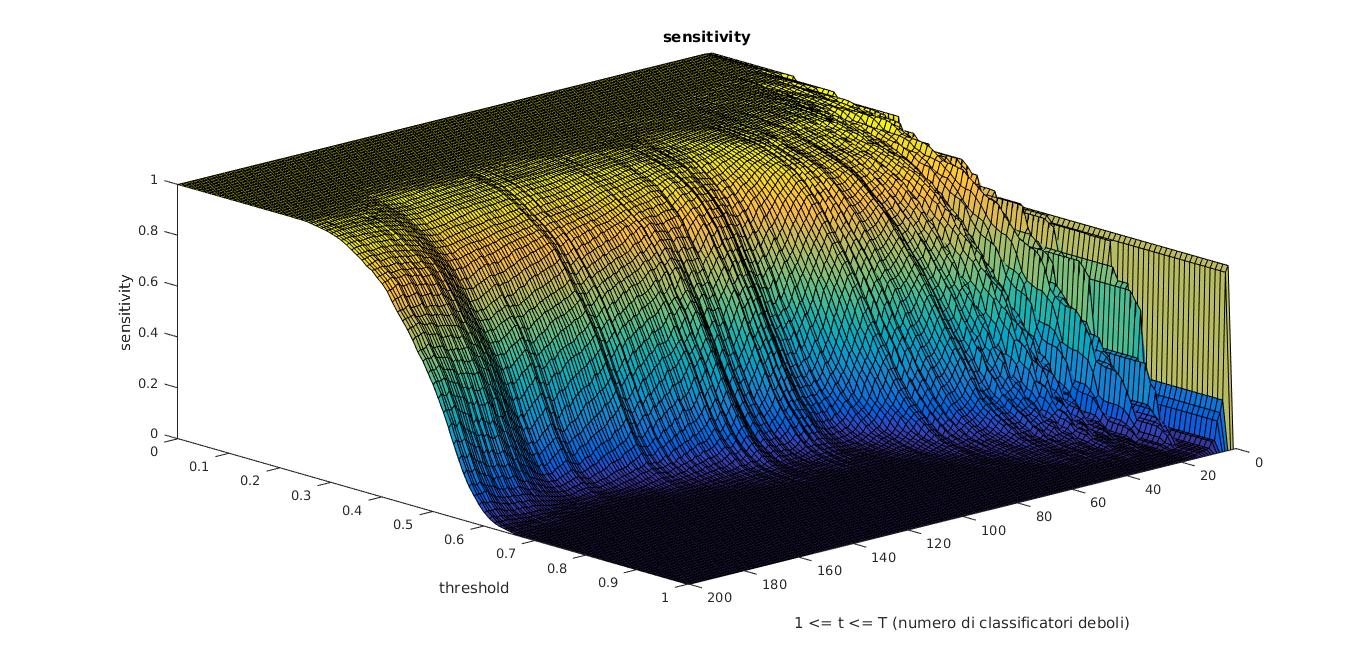
\includegraphics[width=\textwidth]{img/sensitivity_tuning.jpg}
                    \caption{}
                    \label{fig:sensitivity_tuning}
                \end{subfigure}
                ~ %add desired spacing between images, e. g. ~, \quad, \qquad, \hfill etc. 
                  %(or a blank line to force the subfigure onto a new line)
                \begin{subfigure}[b]{0.9\textwidth}
                    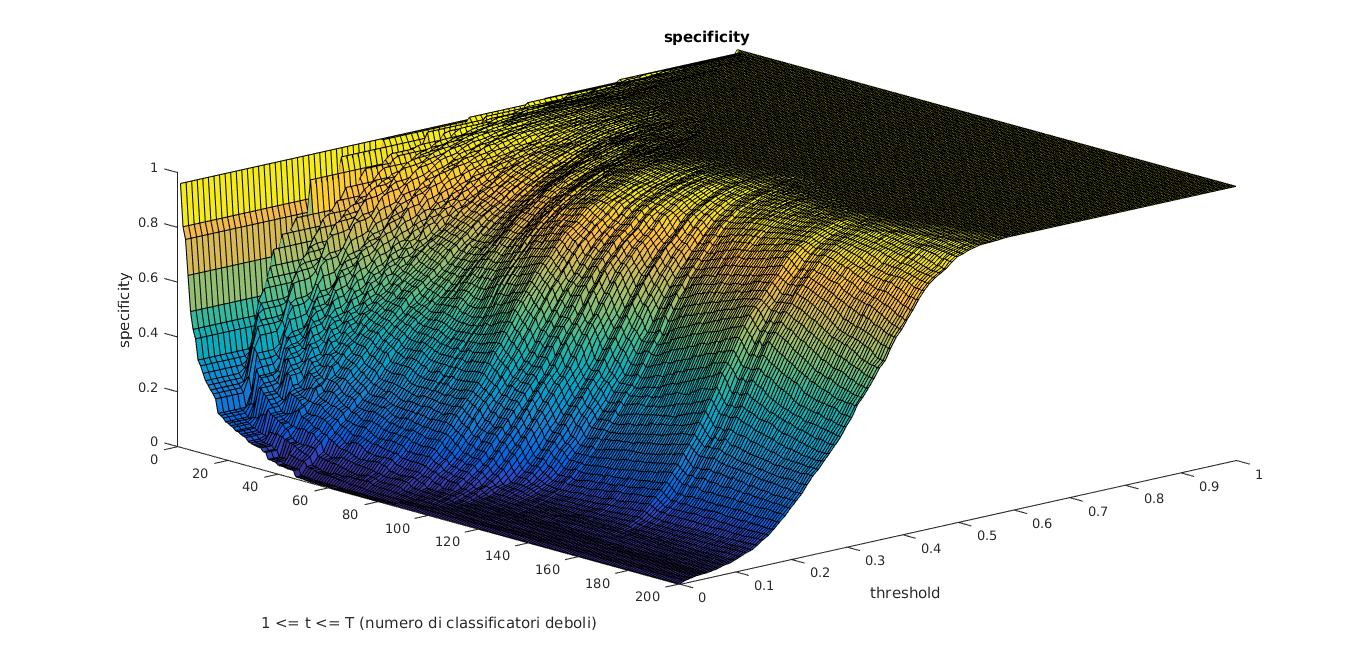
\includegraphics[width=\textwidth]{img/specificity_tuning.jpg}
                    \caption{}
                    \label{fig:specificity_tuning}
                \end{subfigure}
                \begin{subfigure}[b]{0.9\textwidth}
                    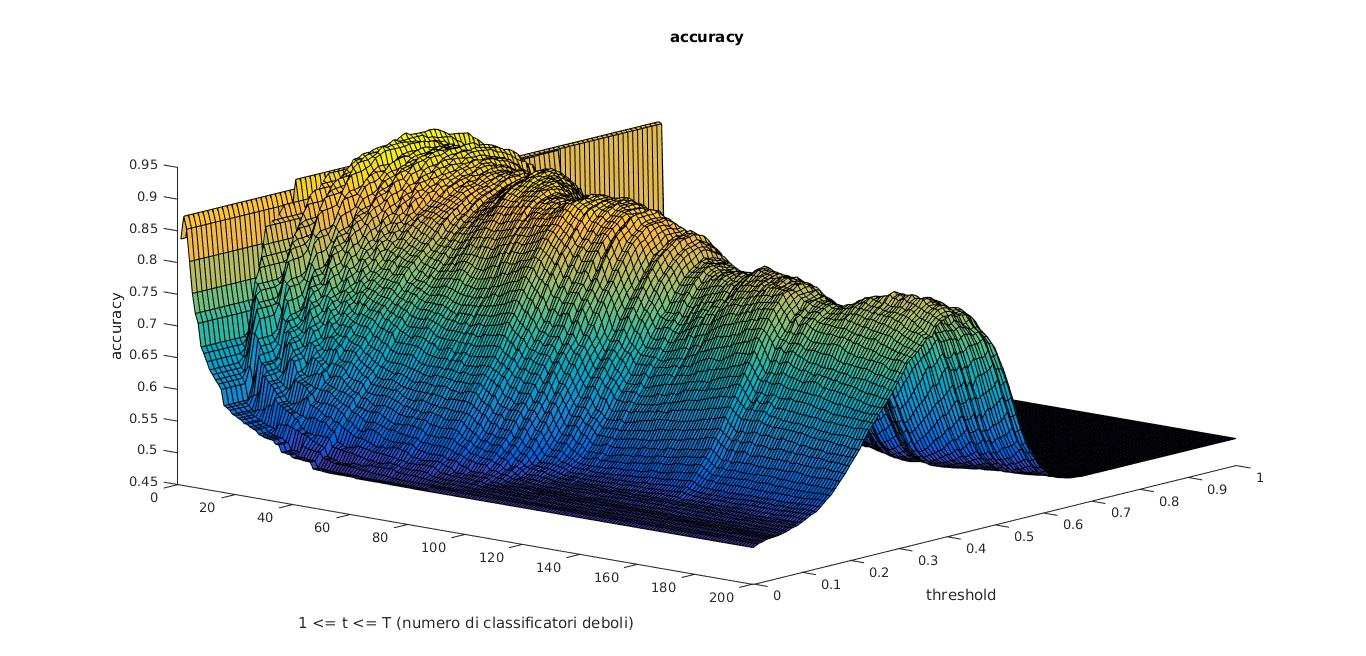
\includegraphics[width=\textwidth]{img/accuracy_tuning.jpg}
                    \caption{}
                    \label{fig:accuracy_tuning}
                \end{subfigure}
                \caption{Plot tridimensionale dell'andamento di \emph{sensitivity} (\ref{fig:sensitivity_tuning}), \emph{specificity} (\ref{fig:specificity_tuning}) e \emph{accuracy} (\ref{fig:accuracy_tuning}) al variare del valore di soglia e del numero di weak learner di $F_{hor}$.}
                \label{fig:performance_evaluation}
            \end{figure}

    \section{Analisi dei Risultati} % (fold)
    \label{sec:analisi_dei_risultati}
        Al termine della procedura di selezione della coppia ottima, si ottiene un classificatore la cui accuratezza è la migliore rispetto a tutte le altre possibili coppie di parametri.

            \subsection{Soglia del classificatore} % (fold)
            \label{sub:soglia_del_classificatore}            
                In letteratura il valore di soglia di un classificatore forte si assume essere pari a 0.5, come descritto da Freund e Schapire in \cite{Freund97}, Viola e Jones in \cite{Viola04}.

                Nel lavoro presentato da Zhu e Wong in \cite{Zhu13}, tuttavia, il valore di soglia non viene esplicitato, ma viene considerato un parametro libero, pur senza fornire alcun metodo esplicativo per la sua derivazione.

                Il valore ottenuto tramite l'algoritmo di massimizzazione dell'accuratezza dei classificatori (sezione \ref{sec:accuracy_maximization}) si aggira intorno al valore $0.4$ per entrambi ($F_{hor}$ e $F_{ver}$).
                
                Una prima interpretazione potrebbe essere la seguente: la discordanza, seppur contenuta, tra il valore di soglia presente in letteratura ed il valore calcolato può essere dovuto a problemi di overfitting al dataset di validazione.
                Senza dover creare un ulteriore dataset esclusivamente per il testing, potrebbe essere utile utilizzare il valore $0.5$ come soglia effettiva dei classificatori finali, eliminando l'overfitting, e considerare le soglie calcolate come delle controprova della correttezza dell'algoritmo di allenamento.

                La seconda interpretazione, invece, è diametralmente opposta: l'aver ottenuto dei valori di soglia ottimi per accuratezza, potrebbe essere un valore aggiunto rispetto alla formulazione generale classica dei classificatori forti.

                Per il momento si assumeranno validi i valori ottimi di soglia appena calcolati, tuttavia sarà solo in fase di rilevamento su frame reali che ci si potrà rendere conto della bontà di tale soluzione.
            % subsection soglia_del_classificatore (end)

            \subsection{Numero di Weak Learner} % (fold)
            \label{sub:numero_di_weak_learner}
                Il numero dei classificatori deboli che compongono ciascun classificatore forte, è molto differente da quello ottenuto in altre applicazioni, prima tra tutte il sistema di riconoscimento dei volti di Viola Jones.

                I classificatori forte di questo sistema sono formati da una decina di classificatori deboli, un numero straordinariamente piccolo se confrontato con i migliaia di weak learner necessari a costruire un classificatore di volti.

                Tuttavia è necessario considerare la diversa natura dei due problemi e i diversi canali di acquisizione dei dati per il riconoscimento. L'immagine di profondità di una persona ripresa dall'alto è una rappresentazione grezza, ma essenziale, dell'individuo ed è incredibilmente povera di informazione se paragonata all'immagine di un volto umano.
                La ricchezza di particolari di un volto, l'incredibile variabilità intraclasse dei volti, per non parlare della fortissima sensibilità delle immagini alle variazioni ambientali (come la luce), rende molto più complesso il problema di riconoscimento. Ecco perchè i classificatori di volti sono cento, mille volte più complessi.

                Per raggiungere elevate prestazioni con il framework di Viola-Jones, infatti, è necessario dividere un classificatore forte in diversi stadi, creando dei classificatori a cascata in grado di scartare nel minor tempo possibile, il maggior numero di oggetti che non corrispondono ai volti umani.

                In questo sistema di rilevamento, tutto questo non è necessario. Un numero così basso di classificatori deboli non è dovuto ad un errore, ma è la conseguenza dell'estrema essenzialità delle immagini di profondità dei profili umani.
                
                Come ulteriore argomentazione, si può pensare alle caratteristiche espresse in linguaggio naturale dell'immagine del profilo della persona: sono solamente tre. 
                Quante ne sarebbero necessarie per esprimere le caratteristiche di un volto umano?
            % subsection numero_di_weak_learner (end)

            \subsection{Sensitivity, Specificity, Accuracy} % (fold)
            \label{sub:sensitivity_specificity_accuracy}
                In base a quanto presente in letteratura, un buon sistema di rilevamento presenta dei valori di \emph{sensitivity} intorno al $90\%$ e di \emph{specificity} intorno al $70\%$.

                Ovviamente tali criteri di giudizio dipendono molto dall'applicazione finale del sistema.
                Esisteranno situazioni più critiche che richiederanno parametri più stringenti, ma in fase sperimentale ci si attiene a questi valori empirici.

                I valori di \emph{sensitivity}, \emph{specificity} e \emph{accuracy} complessivi\footnote{In riferimento al classificatore finale. I singoli classificatori forti, allenati con Adaboost, vengono utilizzati in parallelo in modo da formare uno unico.}, calcolati una volta che i parametri dei classificatori sono stati fissati in condizioni di massima accuratezza, sono i seguenti:

                \begin{equation}
                    \label{eq:sensitivity_value}
                    TPR = 96.87\%
                \end{equation}

                \begin{equation}
                    \label{eq:specificity_value}
                    TNR = 91.25\%
                \end{equation}

                \begin{equation}
                    \label{eq:accuracy_value}
                    ACC = 93.87\%
                \end{equation}

                Alla luce dei risultati ottenuti, il classificatore finale, testato sul dataset di validazione, risulta sufficientemente accurato rispetto ai valori empirici di riferimento.

    % section analisi_dei_risultati (end)